\documentclass[aspectratio=169,usenames,dvipsnames]{beamer}
\usepackage{preamble}
\title{Coding for Humanities, week 2}
\begin{document}

\begin{frame}
    \titlepage
\end{frame}

% Notes:
% - sketch hierarchy on board: list -> sequence -> iterable -> object
% - mention DRY 
\begin{frame}{Plan for today}
    \tableofcontents
\end{frame}

\begin{frame}{Motivation}
    Until now:
    \begin{itemize}
        \item Work with simple values (numbers, text)
        \item Formulas, arithmetic
        \item Store results in memory (variables)
    \end{itemize}

    \pause
    Today:
    \begin{itemize}
        % \item Indexing and slicing strings/lists
        \item Complex values (\lstinline{list})
        \item Making decisions (\lstinline{if})
        \item Repetition (\lstinline{for})
    \end{itemize}
\end{frame}

\section{Sequence types}
\subsection{Strings}
\frame{\tableofcontents[currentsubsection]}

\begin{frame}{Strings}
    \begin{definition}
        A \structure{string}, short for string of characters,
        is a type of value that contains text.
    \end{definition}

\end{frame}

% \begin{frame}[fragile]{Operations on strings}
% \begin{lstlisting}
% In: first = 'John'
% In: last = 'Doe'
% \end{lstlisting}
% \begin{description}
%     \item[first + last] \lstinline{'JohnDoe'}
%     \item[first - last] TypeError
%     \item[first * last] TypeError
%     \item[first / last] TypeError
% \end{description}
%
% \begin{itemize}
% \item + can be used to concatenate two strings
% \item The other operations require numbers, not text
% \end{itemize}
% \end{frame}
%
% \begin{frame}[fragile]{Mixing strings and numbers}
% \begin{lstlisting}
% In: first = 'John'
% In: num = 3
% \end{lstlisting}
% \begin{description}
%     \item[first + num] TypeError
%     \item[first - num] TypeError
%     \item[first * num] 'JohnJohnJohn'
%     \item[first / num] TypeError
% \end{description}
%
% \begin{itemize}
% \item * can be used to repeat a string several times
% \item For the other operations, Python refuses to mix up types
% \end{itemize}
% \end{frame}
%
% \begin{frame}[fragile]{Special characters in strings: `escape sequences'}
% % syntax highlighting is incorrect so disable it
% \begin{lstlisting}[language=]
% In: print("John's bike")
% John's bike
% In: print('John\'s bike')  # single quote
% John's bike
% In: print('John\tMary')    # tab
% John    Mary
% In: print('John\nMary')    # new line
% John
% Mary
% In: print('Backslash: \\')
% Backslash: \
% In: print('up\down')       # \d is not defined, so backslash is kept
% up\down
% In: print("\U0001F923", "\N{grinning face}") 
% [rolling on the floor laughing and grinning emojis ...]
% \end{lstlisting}
% \end{frame}

\begin{frame}[fragile]{Indexing: extracting one element}
\begin{columns}
\column{0.5\linewidth}
\begin{lstlisting}
In: name = 'John'
In: name[0]
Out: 'J'
In: name[-1]
Out: 'n'
\end{lstlisting}
    \begin{itemize}
        \item \lstinline{a[n]} gets the n'th character
        \item Counting starts at 0
        \item negative indices start from the end:\\
            -1 for last character, \\
            -2 second to last, etc.
    \end{itemize}
\column{0.5\linewidth}
    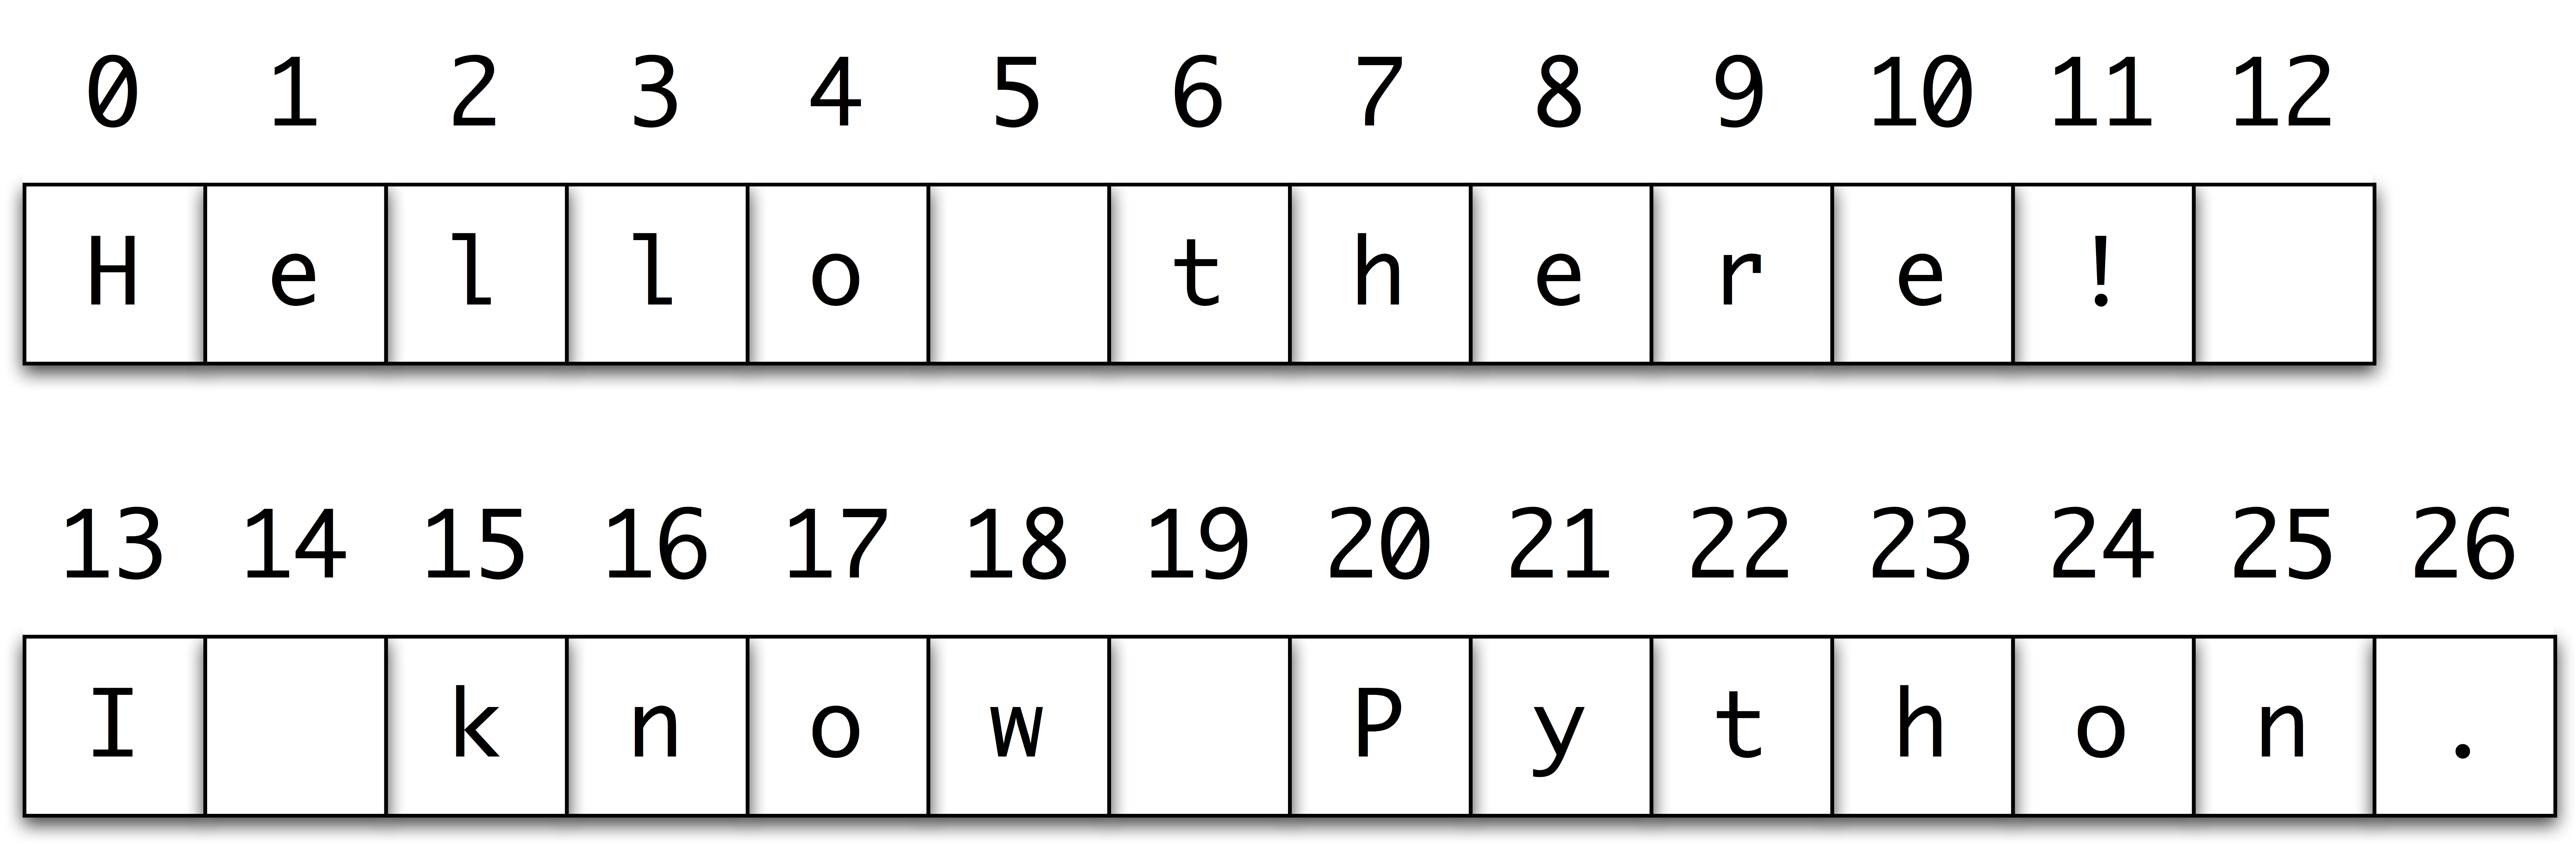
\includegraphics[width=0.9\textwidth]{fig/indexing}
\end{columns}
\end{frame}

\begin{frame}[fragile]{Slicing: extracting a range of elements}
\begin{lstlisting}
In: name = 'John'
In: name[1:3]
Out: 'oh'
In: name[:2]
Out: 'Jo'
In: name[1:]
Out: 'ohn'
\end{lstlisting}
    \begin{itemize}
        \item \lstinline{a[n:m]} extracts characters n to m
        \item Counting starts at 0
        \item Result is up to but not including character m \\
                (half-open interval)
        \item if n or m is left out, beginning or end is used
    \end{itemize}
\end{frame}


\begin{frame}{Indexing and slicing}
    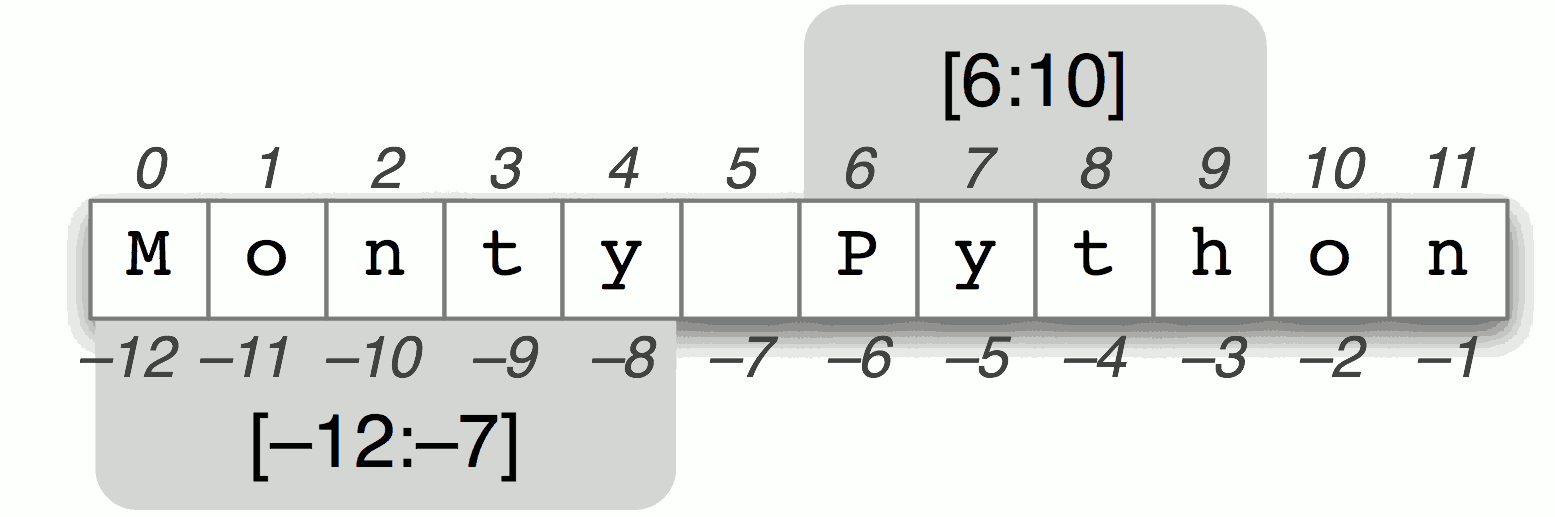
\includegraphics[width=0.8\textwidth]{fig/slices}
\end{frame}

\begin{frame}[fragile]{Length}
Get the number of characters in a string:
\begin{lstlisting}
In: name = 'John'
In: len(name)
Out: 4
\end{lstlisting}
\end{frame}

% \begin{frame}{Refresher: Functions}
%     We have seen builtin \structure{functions}:
%     \begin{itemize}
%         \item \lstinline{int()}
%         \item \lstinline{print()}
%         \item \lstinline{len()}
%     \end{itemize}
%     \pause
%     \begin{definition}
%         A \structure{function} is a piece of code
%         that can be invoked by name.
%
%     \begin{itemize}
%         \item It may take input (arguments): \lstinline{len(name)}
%
%         \item It may produce a result: \lstinline{len(name)} \\
%             or an effect: \lstinline{print('hello', name)}
%
%         \item The notation \lstinline{f(x)} means that the function \lstinline{f}
%             is \structure{applied} to the value \lstinline{x}. \\ 
%             Or simply: \lstinline{f} is \structure{called}.
%     \end{itemize}
%     \end{definition}
%     \pause
%     More about functions next week (including how to make your own)
% \end{frame}

\begin{frame}[fragile]{Format strings}
\begin{lstlisting}
In: x = 1
In: y = 2
In: z = x +  y
\end{lstlisting}
How to combine text and variables in a message?
\begin{lstlisting}
In: print('The sum of ' + str(x) + ' and ' + str(y) + ' is ' + str(z) + '.')
\end{lstlisting}\vspace{-1em}
\begin{lstlisting}[style=plain]
The sum of 1 and 2 is 3.
\end{lstlisting}\vspace{-1em}
\begin{lstlisting}
In: print('The sum of', x, 'and', y, 'is', z, '.')
\end{lstlisting}\vspace{-1em}
\begin{lstlisting}[style=plain]
The sum of 1 and 2 is 3 .
\end{lstlisting}

\pause
Better:
\begin{lstlisting}
In: print(f'The sum of {x} and {y} is {z}.')
\end{lstlisting}\vspace{-1em}
\begin{lstlisting}[style=plain]
The sum of 1 and 2 is 3.
\end{lstlisting}

Simple is better, last method is best.
\end{frame}

\begin{frame}{Sequences}
    Strings are a kind of \structure{sequence}
    consisting of characters.

    \vspace{1em}
    A sequence contains elements in a particular order

    \vspace{1em}
    Operations on sequences:
    \begin{description}[concatenation:]
        \item[getting length:]     \lstinline{len(seq)}
        \item[indexing:]           \lstinline{seq[index]}
        \item[slicing:]            \lstinline{seq[start:end]}
        \item[concatenation:]      \lstinline{seq1 + seq2}
        %\item[repetition:]         \lstinline{seq * num}
    \end{description}
\end{frame}


\subsection{Lists}
\frame{\tableofcontents[currentsubsection]}

\begin{frame}[fragile]{Lists}
    \begin{definition}
    Lists are sequences that may contain any kind of value as items
    \end{definition}
\begin{lstlisting} 
In: numbers = [0, 1, 2]
In: names = ['John', 'Mary']
\end{lstlisting} 
\end{frame}

\begin{frame}[fragile]{List indexing}
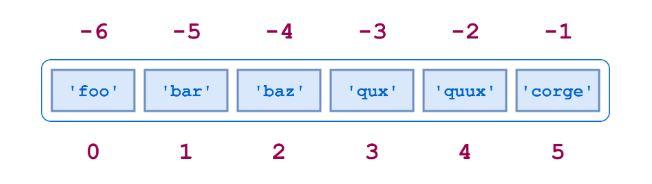
\includegraphics[width=0.9\textwidth]{fig/list}
\end{frame}

\begin{frame}[fragile]{Changing items}
\begin{lstlisting} 
In: names = ['John', 'Mary']
In: names[1] = 'Alice'
In: names
Out: ['John', 'Alice']
\end{lstlisting} 

\pause
NB: cannot change characters in a string (must make new string)
\begin{lstlisting} 
In: name = 'Maria'
In: name[0] = 'D'
\end{lstlisting}\vspace{-1em}\begin{lstlisting}[style=plain]
TypeError: 'str' object does not support item assignment
\end{lstlisting}

Lists are mutable, strings are immutable:
\begin{definition}
An \structure{immutable} object cannot be changed after it is created.
\end{definition}
\end{frame}

\begin{frame}{Why immutable vs mutable?}
    \begin{description}
        \item[Immutable]
            \begin{itemize}
                \item Easier to reason about:\\
                    created once, never modified
                \item Constant values sometimes required\\
                    (dictionaries, next lecture)
            \end{itemize}

        \item[Mutable]
            \begin{itemize}
                \item More efficient with many changes
                \item More 'natural'
            \end{itemize}
    \end{description}
\end{frame}

\begin{frame}{Objects, methods}
    In Python, every value is an object:

    \begin{definition}
        An \structure{object} encapsulates
        data and code for dealing with that data.

        A function that belongs to and operates on an object
        is called a \structure{method}.
    \end{definition}
   
    \begin{description}
        \item[Regular function:] \lstinline{func(a, ...)}
        \item[Method of object:] \lstinline{obj.func(a, ...)}
    \end{description}
\end{frame}

\begin{frame}[fragile]{Adding items}
We can add an item to the end of an existing list:
\begin{lstlisting} 
In: names = ['John', 'Mary']
In: names.append('Alice')
In: names
Out: ['John', 'Mary', 'Alice']
\end{lstlisting}

\pause
We can combine two lists into a new list:
\begin{lstlisting} 
In: friends = ['John', 'Mary']
In: enemies = ['Alice', 'Bob']
In: friends + enemies
Out: ['John', 'Mary', 'Alice', 'Bob']
\end{lstlisting}

\vspace{1em}
NB: \lstinline{append} mutates the list, \lstinline{+} creates a \structure{new} list
\end{frame}


% \begin{frame}[fragile]{Removing items}
% We can remove an item anywhere in a list:
% \begin{lstlisting} 
% In: names = ['John', 'Mary']
% In: names.remove('John')
% Out: ['Mary']
% \end{lstlisting}
%
% \lstinline{remove(elem)} \structure{searches} for the first occurrence of
% \lstinline{elem} and removes it.
%
% \pause
% \vspace{1em}
% Can also remove items at particular positions:
% \begin{lstlisting} 
% In: acquaintances = ['John', 'Mary', 'Alice', 'Bob', 'Max']
% In: acquaintances.pop(3)  # removes 4th item
% In: acquaintances.pop()   # removes last item
% In: friends = acquaintances[:2]  # new list from slice
% In: friends
% Out: ['John', 'Mary']
% \end{lstlisting}
%
% % We can also use slicing to keep a part of a list
% % \begin{lstlisting} 
% % In: acquaintances = ['John', 'Mary', 'Alice', 'Bob']
% % In: friends = acquaintances[:2]
% % In: friends
% % Out: ['John', 'Mary']
% % \end{lstlisting}
% %This is faster if you know where the items are that you want to keep.
% \end{frame}
%
% \begin{frame}[fragile]{Sorting}
% \begin{lstlisting} 
% In: letters = list('ocd')
% In: letters
% Out: ['o', 'c', 'd']
% In: sorted(letters)
% Out: ['c', 'd', 'o']
% \end{lstlisting}
%
% NB: sorted leaves the original list unchanged,
% assign it to keep the result.
% \end{frame}


\begin{frame}[fragile]{Nested lists: lists inside of lists \dots}
    \begin{columns}
        \column{0.3\linewidth}
            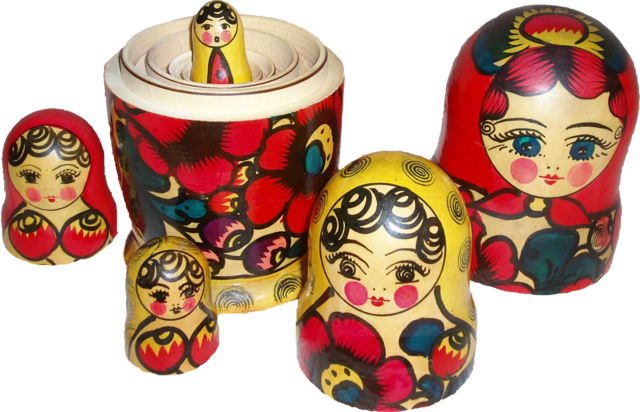
\includegraphics[width=0.95\textwidth]{fig/russiandolls}

            {\scriptsize
            (from \href{https://en.wikipedia.org/wiki/Matryoshka_doll#/media/File:Matryoshka_transparent.png}{Wikipedia})}
        \column{0.7\linewidth}
\begin{lstlisting}
In: ranking = [['John', 1], ['Mary', 3], ['Max', 2]]
\end{lstlisting}

\pause
How to access elements:
\begin{lstlisting}
In: name_and_rank = ranking[1]
In: name_and_rank
\end{lstlisting}\vspace{-1em}\pause\begin{lstlisting}
Out: ['Mary', 3]

In: name_and_rank[1]
\end{lstlisting}\vspace{-1em}\pause\begin{lstlisting}
Out: 3

In: ranking[0][1]
\end{lstlisting}\vspace{-1em}\pause\begin{lstlisting}
Out: 1
\end{lstlisting}
\pause
If we know there will be a fixed sequence of items,
can assign them directly:
\begin{lstlisting}
In: name, rank = name_and_rank
\end{lstlisting}
    \end{columns}
\end{frame}

\begin{frame}[fragile]{Summary: strings vs lists}
Both strings and lists are sequences:
    \begin{itemize}
        \item Items in a fixed order
        \item Has a length
        \item Can extract items or slices
    \end{itemize}

Two important differences:
\begin{enumerate}
    \item lists are more general than strings
        \begin{itemize}
            \item Lists can consist of any data types / objects
            \item Strings always consist of characters
        \end{itemize}
    \item Lists are mutable and strings are immutable
\end{enumerate}

%    Convert between strings and lists:
%        \lstinline{list(), .split(), .join()}
\end{frame}







\section{Making decisions}
\subsection{Conditional expressions}
\frame{\tableofcontents[currentsubsection]}

\begin{frame}{Making decisions: flow charts}
    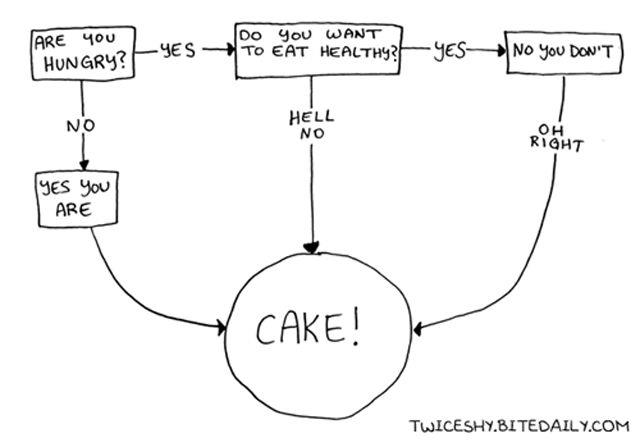
\includegraphics[height=0.8\textheight]{fig/flowchart}
\end{frame}


\begin{frame}{Simple conditions}
    \begin{definition}
        A \structure{conditional expression} is
        an expression that is \lstinline{True} or \lstinline{False}
    \end{definition}
    Conditional operators:
    \begin{itemize}
        \item \lstinline{a == b}: are the values equal?
        \item \lstinline{a != b}: \dots not equal?
        \item \lstinline{a < b}: is \lstinline{a}
                strictly smaller than \lstinline{b}?
        \item \lstinline{a > b}: \dots larger \dots
        \item \lstinline{a in b}: does element \lstinline{a} occur
                in the sequence \lstinline{b}?
    \end{itemize}

    Values and conditions that are \lstinline{True} or \lstinline{False} \\
    are called \structure{Boolean} (George Boole, 1815--1864)
\end{frame}

\begin{frame}{Statements vs expressions}
    NB: == tests equality, \\
           = is an assignment statement!

    \vspace{1em}
    \begin{description}
        \item[Statement:] must occur on a new line. \structure{does} something.
        \item[Expression:] may occur in many places, e.g., inside another expression.
            Evaluates to a \structure{value}, usually without changing anything.
    \end{description}
\end{frame}

\begin{frame}[fragile]{Practical application: testing code}
Conditions can be used to verify that your code works as expected:
\begin{lstlisting}
In: x = 3 * 3
In: print(x == 3 + 3 + 3)
True
\end{lstlisting}

\begin{block}{Useful debugging strategy:}
Sprinkle checks throughout code \\
to confirm whether results match expectations.
\end{block}
\end{frame}


\subsection{Conditional execution: if-statement}
\frame{\tableofcontents[currentsubsection]}

\begin{frame}[fragile]{The if-statement}
\begin{lstlisting}
if books > 5:
    print('you are an avid reader')
\end{lstlisting}

    \begin{itemize}
        \item Code under \lstinline{if}-statement is only executed
            if its condition is \lstinline{True}.
        \item The indentation determines which code is covered
            by the condition
    \end{itemize}

    \pause
    \begin{definition}
        A \structure{code block} is a sequence of lines after
        a statement ending in `:'

        The start and end of the block are defined by the amount of indentation
        (i.e., leading spaces) of the lines.
    \end{definition}
\end{frame}

\begin{frame}[fragile]{if-statement examples}
\begin{lstlisting}
In: books = 6
In: if books > 5:
In:     print('you are an avid reader')
\end{lstlisting}\vspace{-1em}\pause\begin{lstlisting}[style=plain]
Out: you are an avid reader
\end{lstlisting}
\pause
\begin{lstlisting}
In: books = 3
In: if books > 5:
In:     print('you are an avid reader')
\end{lstlisting}\vspace{-1em}\pause\begin{lstlisting}[style=plain]
(nothing)
\end{lstlisting}
\pause
\begin{lstlisting}
In: books = 'many'
In: if books > 5:
In:     print('you are an avid reader')
\end{lstlisting}\vspace{-1em}\pause\begin{lstlisting}[style=plain]
TypeError: '>' not supported between instances of 'str' and 'int'
\end{lstlisting}
\end{frame}


\begin{frame}[fragile]{Optional extensions of the if-statement}
\begin{lstlisting}
if books > 5:
    print('you are an avid reader')
else:
    print('you should read more')
\end{lstlisting}

\begin{itemize}
    \item The code under \lstinline{else} is executed if the condition does NOT match.
    \item Forced choice: necessarily, one of the two options will be executed.
\end{itemize}
\end{frame}


\begin{frame}[fragile]{Optional extensions of the if-statement}
\begin{lstlisting}
if books > 15:
    print('you should get out more')
elif books > 5:
    print('you are an avid reader')
else:
    print('you should read more')
\end{lstlisting}

\begin{itemize}
    \item Can add multiple extra conditions with 'elif' (else if)
    \item The conditions are tested from top to bottom;
            when one of them matches, the rest are ignored.
\end{itemize}
\end{frame}


\begin{frame}[fragile]{Complex conditions}
    Can create complex conditions from other conditions:
    
    \begin{itemize}
        % NB \lstinline does not work inside \item[...]
        % so we don't use a description environment
        \item \lstinline{cond1 and cond2}:
            result is \lstinline{True} if both are \lstinline{True}
        \item \lstinline{cond1 or cond2}:
            result is \lstinline{True} if either or both are \lstinline{True}
        \item \lstinline{not cond}:
            result is \lstinline{True} if \lstinline{cond}
            is \lstinline{False}, and vice versa
    \end{itemize}

    \pause
    For example:
\begin{lstlisting}
if books > 5 and books < 15:
    ...
\end{lstlisting}

\end{frame}

\begin{frame}[fragile]{Truthy and Falsy things}
\begin{itemize}
    \item The number zero and empty sequences are treated as \lstinline{False}.
    \item Nonzero numbers and nonempty sequences are treated as \lstinline{True}.
\end{itemize}

These are equivalent:
\begin{lstlisting}
if len(booklist) != 0:
    print('yes')    
if len(booklist):
    print('yes')    
if booklist:
    print('yes')    
\end{lstlisting}

    Simple is better, so last one is preferred
\end{frame}

\begin{frame}[fragile]{Converting a decision tree into if-statements}
    \begin{columns}
        \column{0.5\linewidth}
            ``Should you stay at a social gathering?''

            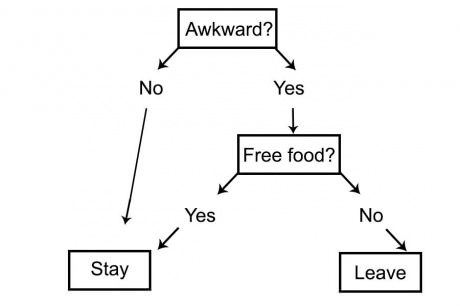
\includegraphics[width=0.8\textwidth]{fig/flowchart2}

        \column{0.5\linewidth}
\begin{lstlisting}
awkward = False
free_food = True
\end{lstlisting}
\pause
\begin{lstlisting}
if awkward:
    if free_food:
        print('Stay')
    else:
        print('Leave')
else:
    print('Stay')
\end{lstlisting}
\end{columns}
\end{frame}


\begin{frame}{Summary: conditions and if}
    \begin{description}[if-statements]
        \item[Conditions] An expression that is \lstinline{True} or \lstinline{False}.
            \begin{description}
                \item[Comparisons, equality tests:] \lstinline{<, >, ==, !=}
                \item[Complex conditions:]          \lstinline{and, or, not}
            \end{description}
        \item[if-statements]
            \begin{itemize}
                \item Execute statements only if condition is True
                \item Indentation matters!
            \end{itemize}
    \end{description}
\end{frame}


\section{Repetition: play it again, Sam!}
\subsection{The for-loop}
\frame{\tableofcontents[currentsection]}

\begin{frame}[fragile]{Repeating statements: for-loops}
\begin{columns}
    \column{0.5\linewidth}
\begin{lstlisting}
booklist = ['a', 'b', 'c']
for book in booklist:
    print(book)
\end{lstlisting}
Result:
\begin{lstlisting}
a
b
c
\end{lstlisting}

    \column{0.5\linewidth}\pause
The loop is equivalent to:
\begin{lstlisting}
book = booklist[0]
print(book)
book = booklist[1]
print(book)
book = booklist[2]
print(book)
\end{lstlisting}
\end{columns}

\begin{itemize}
\item The statements under the for-loop are repeated \\
    for every element in the sequence.
\item At every iteration, \lstinline{book} is assigned
    an element of \lstinline{booklist}
\end{itemize}
\end{frame}

\begin{frame}[fragile]{Looping over sequences}
For loops can be used for anything with multiple items (\structure{iterable}):
\begin{columns}
\column{0.5\linewidth}
\begin{lstlisting}
for letter in 'word':
    print(letter)
\end{lstlisting}
Result:
\begin{lstlisting}
w
o
r
d
\end{lstlisting}
        \column{0.5\linewidth}
\begin{lstlisting}
for number in [0, 1, 2]:
    print(number)
\end{lstlisting}
Result:
\begin{lstlisting}
0
1
2
\end{lstlisting}
\end{columns}
\end{frame}

\begin{frame}[fragile]{Nesting loops inside loops!}
    For loops can contain other for loops (nesting):
\begin{lstlisting}
for number in [1, 2]:
    for letter in 'abc':
        print(number, letter)
\end{lstlisting}
What does the result look like?

\pause
Result:
\begin{lstlisting}
1 a
1 b
1 c
2 a
2 b
2 c
\end{lstlisting}
\end{frame}



\begin{frame}[fragile]{Looping without a list}
Can use the \lstinline{range} function
if we don't have a list:
\begin{lstlisting}
for number in range(4):
    print(number)
\end{lstlisting}

Result:
\begin{lstlisting}
0
1
2
3
\end{lstlisting}

Repeats 4 times. Last item is 3 because counting starts at 0.
\end{frame}


\begin{frame}{Summary}
    \begin{description}
        \item[for-loop] repeat code for each element
        \item[iterables] \lstinline{str, list, range}
    \end{description}
\end{frame}

\section{Example problems and solutions}
\subsection{Counting letters}
\frame{\tableofcontents[currentsection]}

\begin{frame}[fragile]{Example}
How to count the number of `a's in a string?
\begin{lstlisting}
word = 'banana'
count = 0
\end{lstlisting}
\pause
\begin{lstlisting}
for letter in word:
    if letter == 'a':
        count += 1
print(count)
\end{lstlisting}
\end{frame}


\subsection{Reversing text}
\begin{frame}[fragile]{Reversing text}
Write code that computes the reversal of a string.

   \vspace{1em}
   For example, the string \lstinline{'I am testing'} should result in
   \lstinline{'gnitset ma I'}.

\begin{lstlisting}
string = 'I am testing'
result = ''
\end{lstlisting}
\pause
\begin{lstlisting}
for letter in string:
    result = letter + result
print(result)
\end{lstlisting}

\pause
Shorter solution:
\begin{lstlisting}
print(string[::-1])
\end{lstlisting}
\end{frame}


\subsection{Palindromes}
\begin{frame}[fragile]
Write code that recognizes palindromes
   (i.e. words that look the same written backwards).

   \vspace{1em}
    For example, \lstinline{'radar'} is a palindrome, but \lstinline{'radio'} is not.

\begin{lstlisting}
string = 'radar'
\end{lstlisting}
\pause
\begin{lstlisting}
backwards = string[::-1]
print(backwards == string)
\end{lstlisting}
\end{frame}
 
\subsection{Overlapping lists?}
\begin{frame}[fragile]
    Write code that takes two lists and checks if they have \emph{at least} one
    member in common.

    \vspace{1em}
    You may use the \lstinline{in} operator, but for the sake of the
    exercise, you should (also) write it using two nested for-loops.
\begin{lstlisting}
list1 = [1, 2, 3]
list2 = [1, 4, 6]
overlapping = False
\end{lstlisting}
\pause
\begin{columns}[T]
\column{0.47\linewidth}
\begin{lstlisting}
for elem1 in list1:
    for elem2 in list2:
        if elem1 == elem2:
            overlapping = True
print(overlapping)
\end{lstlisting}
\pause
\column{0.47\linewidth}
Shorter:
\begin{lstlisting}
for elem1 in list1:
    if elem1 in list2:
        overlapping = True
print(overlapping)
\end{lstlisting}
\end{columns}
\end{frame}

\begin{frame}{Summary of today}
    \begin{description}[Sequence types]
        \item[Sequence types] strings and lists
        \item[Conditions] if-statement
        \item[Repetition] for-loop
        \item[Nesting]
            \begin{itemize}
                \item lists inside lists
                \item if-statements inside if-statements
                \item for-loops inside for-loops
            \end{itemize}
    \end{description}
\end{frame}


\begin{frame}{Readings and lab}
    \begin{itemize}
        \item Finish ch.~2 of Introduction to Cultural Analytics,\\
            \url{https://melaniewalsh.github.io/Intro-Cultural-Analytics/}
        \item Notebook ch.\ 2
        \item Exercises
    \end{itemize}
\end{frame}
\end{document}
